\chapter{Implementation}\label{C:imple}


//TODO rename sections to reflect work done
\section{Mechanical Design}

\subsection{Rotating Pipette Mount}

\subsection{Z micrometer Control}

\section{Software}

\subsection{Motorised Dispensing Controller}
ESP32 based system controller with serial interface for issuing commands. Provides functionality to:
\begin{itemize}
    \item Motorised stages, height and angular position
    \item e-Pipette droplet dispensing 
\end{itemize}

\subsection{Environmental Monitor}
\subsection{Temperature Logger}

\section{Electronic Design}

\subsection{Motor Driving}

\subsection{Setup and Requirements}
//TODO rewrite

Driving firmware was implemented on an ESP32 to validate its ability in producing the required pulse train step signal. The controller was required to produce N steps (pulses) at a set average speed, and ramp up and down that pulse speed at the head and tail of that signal.

Set values of 200 steps forward and back, at a speed of 200 steps per second, with max acceleration or 800 steps per second per second:

These pulses were captured on a second microcontroller listening for falling edges to trigger an interrupt routine to record and display that data.

\subsection{Results}

Figure \ref{fig:code}:a shows a successfully produced signal of 200 pulses with an inferred acceleration at its head/tail. This speed ramping is better illustrated in figure \ref{fig:code}:b showing the stepping change in pulses per second over the course of the pulse train.

\begin{figure}[h]
    \centering
    \begin{subfigure}{.45\textwidth}
        \centering
        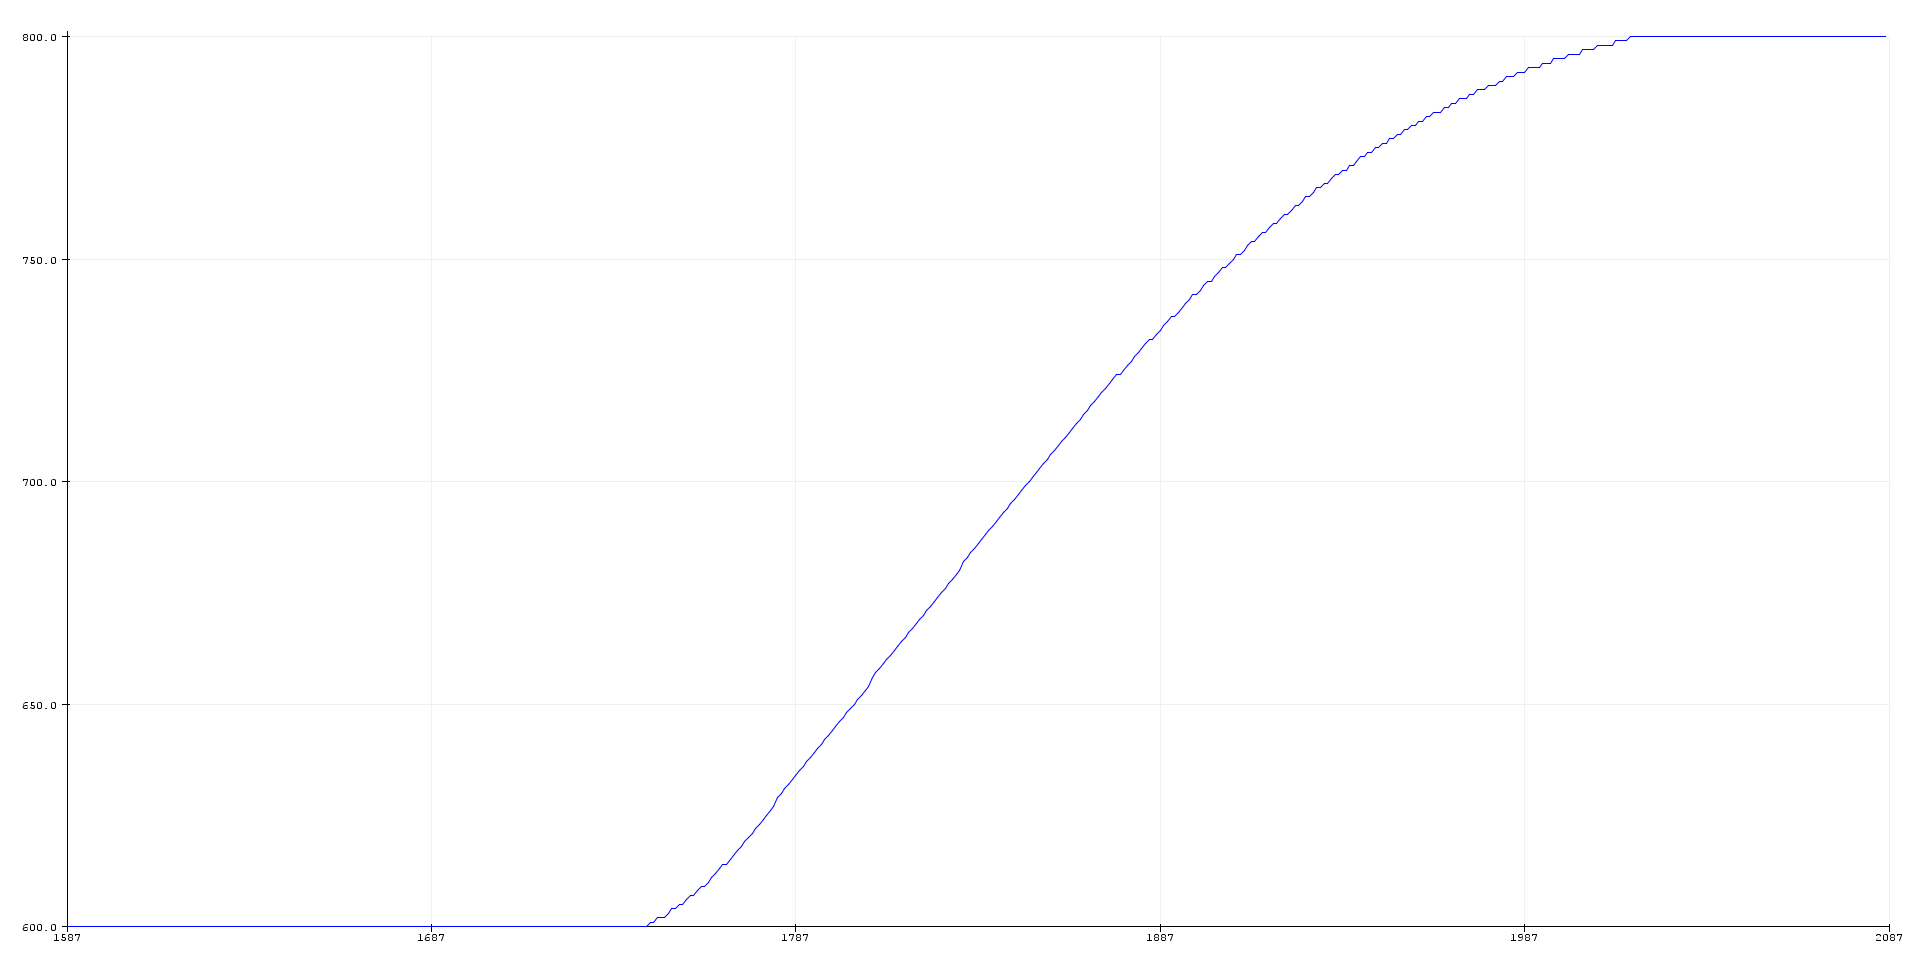
\includegraphics[width=0.8\linewidth]{img/stepper_pulses.PNG}
        \caption{Pulse Count}
    \end{subfigure}%
    \begin{subfigure}{.45\textwidth}
        \centering
        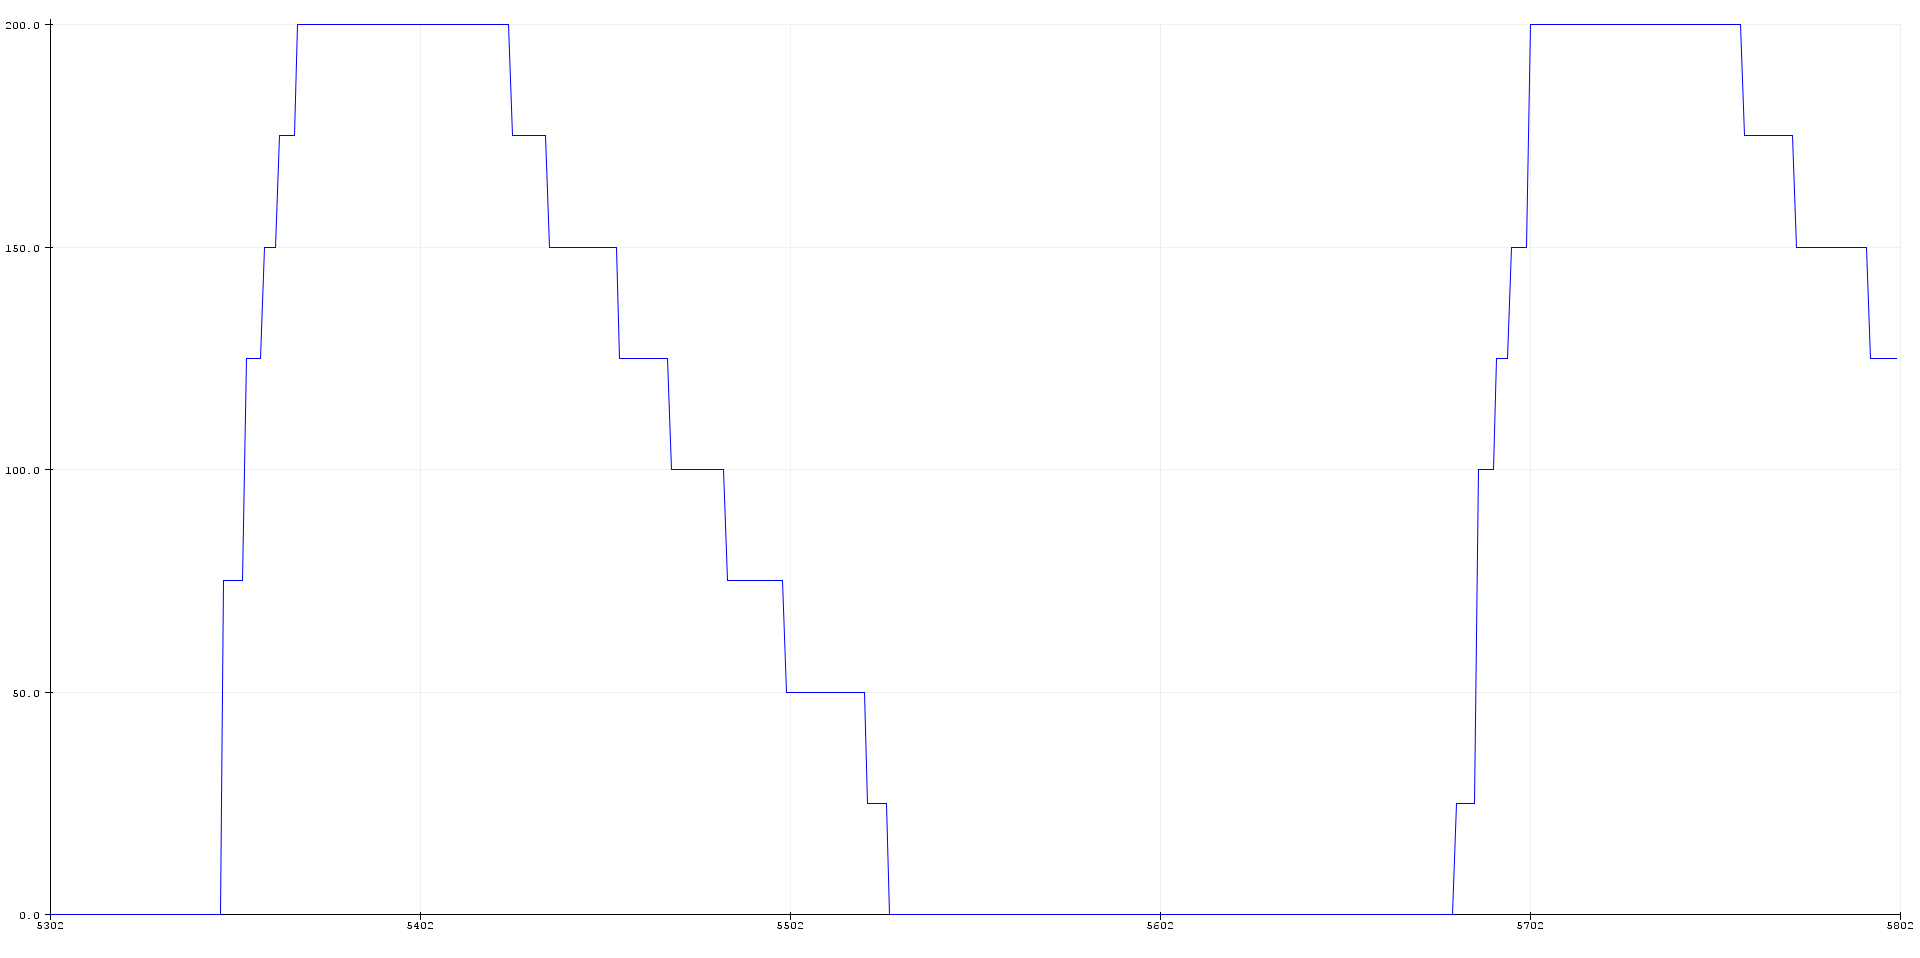
\includegraphics[width=0.8\linewidth]{img/stepper_pulse_acc.PNG}
        \caption{Pulses per Second}
    \end{subfigure}
    \caption{}
    \label{fig:code}
\end{figure}

\subsection{Pipette Triggering}

\subsection{Environmental Monitoring}
